\subsection{2.2 Matrixmultiplikation}{
\vskip1pt
Matrizen können auf folgende Weise miteinander multipliziert werden:

\begin{center}
\fbox{
$A \cdot B = C \hspace{5pt} \Rightarrow \hspace{5pt} c_{ik} = \sum_{j=1}^n a_{ij} \cdot b_{jk}$
}
\end{center}

\vspace{-2mm}

\begin{center}
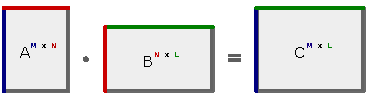
\includegraphics[width = 0.95 \columnwidth]{2_Matrizen/Matrixmultiplikation.pdf}
\end{center}



\textbf{Assoziativ- \& Distributivgesetz:}

\vspace{-6mm}
\begin{center}
\parskip3pt
\begin{align}
(A\cdot B) \cdot C &= A \cdot (B \cdot C) \nonumber \\
(A + B) \cdot C &= A \cdot C + B \cdot C \nonumber \\
A \cdot (C + D) &= A \cdot C + A \cdot D \nonumber
 \end{align}
\end{center}
\textbf{Achtung!} Kommutativgesetz gilt nicht! i.A. $A\cdot B \neq B \cdot A$
}
\WhiteSpace